\section{Approach}
\label{sec:approach}

\begin{figure*}[th]
\centering
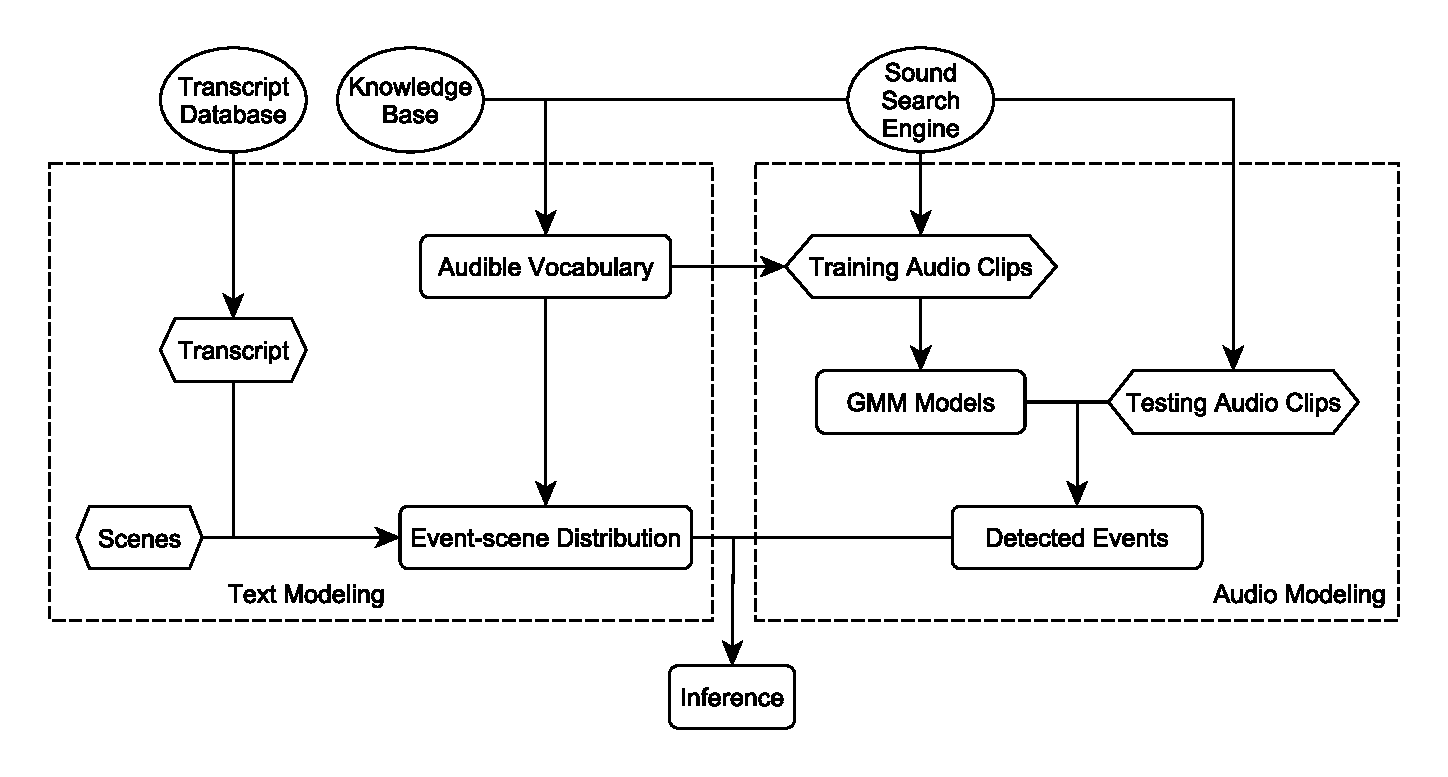
\epsfig{file=figures/all.eps, width=1.6\columnwidth}
\caption{The Auditory Scene Recognition Framework}
\label{fig:sys}
\end{figure*}

Our ASR framework can be roughly divided into two parts: the {\em text 
modeling} and the {\em audio modeling}. In the text modeling part, we seek to
derive probability distribution of predefined auditory scenes given 
a primitive audible event concepts. For example, the probability
distribution conditioned on event ``car'' may be 
\begin{eqnarray*}
Pr(street | car) &=& 0.6\\ 
Pr(station | car) &=& 0.2\\
Pr(park | car) &=& 0.18 \\
Pr(cafe | car) &=& 0.02
\end{eqnarray*}
We obtain such probability distribution by first 
collecting a vocabulary of audible event
concepts such as ``car honk'' and ``engine'', and then by mining the 
relationships between these concepts and the scene terms from large 
volume of text corpus, in particular, movie and TV drama transcripts. 
In the audio modeling part, we first download audio samples of all audible
events from our vocabulary and then train Gaussian Mixture Models (GMMs)
for each event using the corresponding samples. 
During the end-to-end scene recognition phase, the input audio clip 
is automatically segmented into pieces, and passed to an inference engine,
which infers the probability distribution on events for each segment.
Finally, based on the event-scene relations obtained in the text modeling part,
the engine determines the most likely scenes.
\fig{sys} shows an overview of our system. Next, we describe the above 
components of our framework in more detail. 

%Firstly, we build a probability model of events and scenes from drama scripts. Next, using some knowledge base and sound search engine, we can build a word set of audible event. Then we focus on this audible set and download some related audio clips as training data. At the same time, we can label these audio clips automatically using the key words in searching. After that, for
%each event, we train GMM classifiers using ZCR and MFCC as features, in order to detect audible event from audio clips. Finally, we can get the result by combining the detection result and the probability model of events and scenes.
%
%Text part
\subsection{Build Vocabulary of Audible Concepts}
\label{sec:vocab}

\begin{table}
\centering
\caption{Possible Audible Event Terms from Probase}
\label{tab:audible}
\begin{tabular}{|l|l|} \hline
%\multicolumn{2}{|c|}{Probase} 	\\ \hline
{\bf Concepts} & {\bf Entities} \\ \hline \hline
sound & barking dog, music, {\em classical}\\ \hline
noise & siren, traffic, {\em light} \\ \hline
animal & dog, cat, snake	\\ \hline
sound effect & chorus, gunshot, {\em delay}\\ \hline
musical instrument & 	guitar, oboe, trumpet \\ \hline
%\multicolumn{2}{|c|}{WordNet} 	\\ \hline
%sound & voice, ring, unison	\\ \hline
%noise & clack, howl, thunder	\\ \hline
\end{tabular}
\end{table}

We create the audible concept vocabulary by an automatic bootstrapping process.
Each iteration involves a ``growing phase'', which enlarges the 
current pool of audible concepts by including
additional terms from both an online sound search engine and a knowledge base,
and a ``filtering phase'' which removes some of the 
terms which are deemed inaudible from the current pool, 
using the same sound search engine.
The iterations stop when no new terms can be added after the filter phase. 
The final pool of concepts become the vocabulary of audible events.

The knowledge base we use for this purpose is called
Probase\cite{wu2012probase}, which is a probabilistic taxonomy of terms
organized in hypernymy-hyponymy
(isA) relations\footnote{Hypernymy relation, also known as
concept-entity relation, is the most 
important relation in Probase, but there are other relations as well.}.
%and WordNet\cite{miller1995wordnet}. 
Each isA pair ($c$, $e$)\footnote{Here $c$ stands for a concept and
$e$ stands for an entity and the two are related by isA relation: $e$ isA $c$.} 
is associated with a frequency which is the
number of evidences that support this isA relation in a large text corpus, 
and two probability scores known as typicality, defined by
$P(e | c)$ and $P(c | e)$, which are calculated from the statistics of the
occurrences of terms $e$ and $c$ in the corpus.

We start the bootstrapping process by creating an initial pool of
seed candidate event terms. These initial terms were the $k$ most typical
hyponyms (by typicality $P(e | c)$)
under the terms such as ``sound'', ``noise'', ``musical instruments'',
etc.  \tabl{audible} gives the some examples of these candidate audible events 
terms discovered from Probase. One can see that not all of these terms
are truly audible events (those italicized terms in the table). 
We will remove such noises in the later filtering phase, which is described
in the following.

In the {\bf growing phase}, we enrich the current pool by adding related terms
from two sources. We first query a sound search engine
for each existing terms in the pool. The resulting clips for each query
(e.g., ``hunt dog'') carry tags such as ``labrador'' and ``puppy''. 
We represent each new candidate term by its superconcepts in Probase, 
which form a vector. For example, the superconcepts of ``hunt dog'' are 
``dog'', ``animal'', etc. All such terms that exist in Probase as entities 
(i.e., as $e$ in an isA pair) and are not already in the current pool 
are considered new candidates. 
Then we cluster these vectors together by cosine similarity as 
the semantic distance. For each cluster of terms, which presumably 
represent one type of similar objects, we identify their most popular 
super concept as their common ``type''. For example, hunting
dog, labrador and puppy may be clustered together and their common type 
is ``dog.''  Subsequently, other entities under ``dog'', such as 
``police dog'' maybe included in the candidate pool, effectively ``growing'' 
the pool.
%We further expand the set of new candidates 
%by clustering them under different super-concepts. Here is the process.
%During clustering, we represent each
%new term as a vector of its super-concepts in Probase and compute distance
%between any two by Cosine similarity. This way, we could group different 
%variants of dogs together under the concept ``dog''. Since these variants
%are probably audible, we deduce that other entities under ``dog'' are also
%audible, and therefore add the most typical entities under ``dog'' which
%are not in the pool as new candidate terms as well. 
\fig{expand} illustrates this process.

\begin{figure}[th]
\centering
\epsfig{file=figures/expand.eps, width=\columnwidth}
\caption{Expansion using Probase}
\label{fig:expand}
\end{figure}

In the {\bf filtering phase}, every new candidate term from this iteration
is searched in the sound search engine. We look at the information of the
returned audio clips for each term. All clips which are shorter than 0.1 seconds
or longer than 30 seconds are removed, because these are usually not a single
event from our experience. Finally we filter out terms which have
fewer than 10 resulting clips, and keep the rest in our pool and go on to
the next iteration. 


\subsection{Build Event-Scene Probability Model}
\label{sec:mapping}
This section decribes how to compute the conditional probability 
$P(scene | event)$, for the given $n$ scenes in question and all 
terms in the event vocabulary. We first extract fragments of text
corresponding to the input scenes 
from large number of TV drama or movie transcripts, and then extract
audible events from the text. Finally we compute the probability model
between events and scenes. 

\subsubsection{Extraction of Scene Contexts}
In this paper, we choose to use movie and TV drama transcripts 
\footnote{Movie scripts were downloaded from \url{http://www.imsdb.com},
while TV series transcripts were downloaded from 
\url{http://simplyscripts.com/tv.html}.} as 
our primary source to obtain the event-scene relations,
because i) they contain large number of interesting scenes; and ii)
most of them mark clearly the boundaries of a scene, such as those
in \fig{ET}.
%We can make use of such patterns to extract the text context of a scene such
%as ``street.'' as well as its noun synonyms,  e.g., ``avenue'' and 
%``boulevard.'', from WordNet \cite{miller1995wordnet}.
%In addition, because event terms that occur in human conversations 
%are not necessarily events that happen
%in that scene, we remove all conversations which also have clear patterns
%from the context.
%\tabl{scripts} shows a subset of
%dramas and movies which were considered as data sources

%\begin{table}[th]
%\caption{Selected Movies/TV Transcripts}
%\label{tab:scripts}
%\centering
%\small
%\begin{tabular}{llr}
%\toprule
%Title & Type & Length\\
%\bottomrule
%\rowcolor[gray]{.8} The Big Bang Theory & TV & 126 episodes  \\
%					Friends & TV & 229 episodes  \\
%\rowcolor[gray]{.8} How I Met Your Mother & TV & 135 episodes  \\
%					Prison Break & TV & 23 episodes  \\
%\rowcolor[gray]{.8} Lost & TV & 118 episodes  \\
%					Sherlock & TV & 6 episodes  \\
%\rowcolor[gray]{.8} Family Guy & TV & 104 episodes  \\
%					South Park & TV & 232 episodes  \\
%\rowcolor[gray]{.8} Arrested Development & TV & 22 episodes  \\
%					Scrubs & TV & 150 episodes  \\
%\rowcolor[gray]{.8} Modern Family & TV & 84 episodes  \\
%					House M.D. & TV & 177 episodes  \\
%\rowcolor[gray]{.8} Supernatural & TV & 167 episodes  \\
%					The Vampire Diaries & TV & 82 episodes  \\
%\rowcolor[gray]{.8} Firefly & TV & 11 episodes  \\
%					True Blood & TV & 34 episodes  \\
%\rowcolor[gray]{.8} Seinfeld & TV & 179 episodes  \\
%					Wall-E & Movie & 97 minutes  \\
%\rowcolor[gray]{.8} V for Vendetta & Movie & 132 minutes  \\
%					Twilight & Movie & 121 minutes  \\
%\rowcolor[gray]{.8} Toy Story & Movie & 81 minutes  \\
%					Titanic & Movie & 194 minutes  \\
%\rowcolor[gray]{.8} Kung Fu Panda & Movie & 92 minutes  \\
%					King-Kong & Movie & 187 minutes  \\
%\rowcolor[gray]{.8} I am Sam & Movie & 132 minutes  \\
%					The Avengers & Movie & 142 minutes \\
%\rowcolor[gray]{.8} Avatar & Movie & 162 minutes  \\
%					2012 & Movie & 158 minutes  \\
%\rowcolor[gray]{.8} 500 Days Of Summer & Movie & 95 minutes \\
%					E.T. & Movie & 115 minutes  \\
%\bottomrule
%\end{tabular}
%\end{table}

\begin{figure}[th]
\centering
\fbox{\parbox{\columnwidth}{
\small
%\begin{verbatim}
%...
%Elliott and Mike walk down the driveway.\\ 
%They are on their way to school.\\
...They discuss E.T., arguing about how smart he is.

[This is just a transition scene.]\\
EXT: STREET: DAY\\
Mike and Elliot walk towards a bus stop ...
%a group of children are waiting. \\
%Mike's friends torment Elliott about his "goblin."
%...
%\end{verbatim}
}}
\caption{A Snippet from the Transcript of Movie E.T.}
\label{fig:ET}
\end{figure}


%They not only describe what happend in a context, but also present this information in a good manner. In well-written transcripts, when plot switchs, there is a particular sentence in a certain pattern indicating current context, such as "CUTS TO: Captain Raydor's Office" or "Scene: Outlets in Los Angeles". This make it easy to extract the context from a short sentence and help us collect events for contexts accurately.
%
%We use 30 hot American tv series, as shown in \tabl{scripts}.



\subsubsection{Extraction of Events from Contexts}
\label{subsec:lists}
Contexts extracted in \fig{ET} may contain event terms such as ``walk'',
``bus'' and ``children'' that find exact match in our vocabulary.
The vocabulary also contains compound terms such as ``open door'', 
``ring bell'' which may not find exact match in the context. To extract
as many events as possible from the context, besides exact matches for
terms in the vocabulary, we also parse the context using a
dependency parser, and pay special attention to the following relations:
{\em direct object}, {\em indirect object}, {\em noun compound modifier},
{\em nominal subject} and {\em passive nominal subject}.
Each of these relations relates either a noun and a verb, or between
two nouns. The reason we focus on these dependencies is that sound is generally
made by a motion or action and its agent or recipient (single verb or 
verb-noun cases) 
or some object (single noun or noun-noun cases such as ``coffee cup'') alone. 
A word pair $(w_1, w_2)$
with the above five relations from the context is considered an audible
event, if there is a compound event term $w_1w_2$ or $w_2w_1$ in the 
vocabulary. 
 
%
%\begin{enumerate}
%\item Use Stanford NLP to conduct sentence splitting, POS tagging and lemmatization and dependency analysis.
%\item Check all nouns in first sentence (indicating sentence) to see if there is any noun each context's synset . If yes, we label this paragraph with the context.
%\item Based on result provided by POS tagging, we record noun lists and verb lists with frequency, respectively. For multi-word nouns, we just keep the last word, e.g, "safe-guard" becomes "guard".
%\item Analyze the sentence dependency and extract direct object pairs. Each pair is combined alphabetically with space.
%\item Merge noun, verb and pair lists with context same label, respectively. As far, for each context, there are three event lists.
%\item Audible concept set bulit in\ref{subsec:buildingvocabulary} and the three lists intersect to pick out events we concern about.
%\end{enumerate}
%

\subsubsection{Event-scene Distribution}
Our problem is to classify an input audio clip into one of $n$ predefined
scenes. The intuition is that humans recognize a scene by its most important,
and distinctive events. We model this by $P(scene | event)$. For example, if
flushing the toilet is a very distinctive event for the scene ``toilet'', 
then we expect $Pr(toilet | flush)$ is significantly higher than 
$Pr(other\_scene | flush)$.

We compute the probability as
\begin{equation}
\label{eqn:prob}
Pr(scene=s | event=e)  = \frac{TF(s, e)}{\sum_{s \in S} TF(s, e)},
\end{equation}
where $s$ is a scene in the set of $n$ input scenes $S$, 
$e$ is an event in the vocabulary, and $TF(s, e)$ is the number of occurrences
of $e$ in the context of scene $s$.

%Now, we get events and its frequency of each context. Since we assume human beings recognize context audio by catching some notability events, we hope there are some typical events existing in every context, e.g, when there is the sound of toilet flushing, we can barely deny that it is in toilet. So we calculate and normalize TF (term-frequency) of each event, and then filter by it.
%So far, we get the event-context model according to \eqn{model}.
%\begin{equation}
%\label{eqn:model}
%p(scece_j|event_i) = tf_{i, j}
%\end{equation}


%Audio part
\subsection{Train Models for Audible Events} 
\label{sec:audiotrain}

Once we download audio samples for each of the event terms in the vocabulary,
we can train audio models for each event. 

\subsubsection{Feature selection}
To train audio models, first we need to find a good way (features) 
to describe the audio data. 
%Many features have been proposed by researchers in the past. 
We view an audio clip as a sequence of logically overlapping frames, 
each comprised of fix number of sample points, as in \fig{fra}.
The amount of overlap is a parameter of the model.
A frame is the basic unit of feature extraction, 
in either time or frequency domain. 

\begin{figure}[th]
\centering
\epsfig{file=figures/frame.eps,width=0.8\columnwidth}
\caption{Overlapping Audio Frames}
\label{fig:fra}
\end{figure}

%Existing works \cite{1561288,1621215,mitrovic2010features,4761905} reported
%that, in the frequency domain, the mel-frequency cepstrum coefficients (MFCC) 
%feature is a widely-used feature which is a cepstral representation 
%of the audio clip, i.e., a non-linear spectrum-of-a-spectrum. 
%It is fairly robust because it closely resembles the human auditory system's
%response to different frequency bands.
%
%In the time domain, short-time energy is the energy measure of a short segment
%of sound. It has been shown to be a simple and 
%effective feature to distinguish active voice against silence in
%speech processing \cite{1181092}. 
%
%Zero crossing rate (ZCR) is a temporal feature which measures the rate 
%at which the signal transits from positive to negative or back. 
%ZCR can be used to distinguish meaningful events from environmental noise, 
%since environmental noise usually has a larger ZCR.
%
%In our work, we use short time energy to remove ambient noises first. 
%Then, we combine ZCR and MFCC as features, which will be used in the
%audible events modeling next.
%
%\subsubsection{Model selection}
%GMM and HMM are mostly used in these kind of problems. We will discuss both of them in the following sections.

\subsubsection{Event models}
In this paper, every audible event in the vocabulary is modeled as one or
more GMMs. A GMM is a weighted sum of $M$ Gaussian density function, 
which is given by:
\begin{equation}
P(\mathbf{x}|\mathbf{\Theta}) = \sum_{i = 0}^{M - 1} c_i\prod_{d=0}^{D-1} \frac{1}{\sqrt{(2\pi)}\sigma_{i,d}}e^{-\frac{1}{2\sigma_{i,d}^{2}}(x_d-\mu_{i,d})^2},
\label{eqn:gmm}
\end{equation}
where $\mathbf{x}$ is a $D$-dimensional variable representing
the feature vector, $\Theta$ is the parameters of GMM, 
including $\mathbf{c}$, $\mathbf{\mu}$ and $\mathbf{\sigma}$.
$c_i$ is the weight of the $i^{th}$ mixture, with the following constraint:
\begin{equation}
\sum_{i=0}^{M-1}c_i=1,
\end{equation}
while $\mu_{i,d}$ and $\sigma_{i,d}$ are the mean and standard deviation 
of the dimension $d$ of the $i^{th}$ mixture.

\subsubsection{Model training}
The audio samples downloaded for each event term in the vocabulary, 
such as ``dog'' may sound very different, either because there are various
aspects of an event, or in the case of ``dog'', simply because there are
different species -- {\em bull dogs} certainly sound very 
different from {\em chihuahuas}.
To accurately models each event, in this paper, we aim to derive multiple
GMMs, each for a separate aspect of an event. 

Before we do the actual training, we first remove ambient noise from
the training clips. We compute the short time energy \cite{1181092} 
for each frame of the sample:
\begin{equation}
\overline{E} = \frac{1}{N}\sum_{i=0}^{N-1}x^2(i),
\label{eqn:en}
\end{equation}
where $N$ is the number of sample points in a frame, 
%which is set to 512 here, 
and $x(i)$ is the value of $i^{th}$ sample point. 
We only retain the frames with energy higher than average among all
frames. The contiguous frames after the noise removal become segments
within the event. We then remove tiny segments which are shorter than 100ms,
and further split longer segments into 500ms-long pieces.
We believe these resulting segments may carry different
aspects of the same event.

Next we put all remaining segments from all audio samples of 
the same event together and cluster them.
%There are lots of previous work focus on this problem \cite{4587600}. 
We train an interim GMM for each segment using KL divergence 
\cite{kullback51:KL} as a distance measure for clustering.
GMM is trained by EM algorithm: 
\begin{equation}
\label{eqn:pp}
P(\mathbf{O}|\mathbf{\Theta}) = \prod_{i=0}^{L - 1}
P(\mathbf{O_i}|\mathbf{\Theta}).
\end{equation}
where $\mathbf{O_i}$ is the feature vector for frame $i$ combining
zero crossing rate (ZRC) and mel-frequency cepstrum coefficients (MFCC) 
features \cite{1561288,1621215}, and $L$ is the number of frames in the segment. 
ZRC is calculated as:
\begin{equation}
\overline{Z} = \frac{1}{2(N - 1)}\sum_{i=0}^{N-2}(|sgn(x(i)) - sgn(x(i + 1))|),
\end{equation}
where
\begin{equation}
sgn(x) = \left\{\begin{array}{ll} 1 & x\geq 0\\ -1 & x < 0\end{array}\right.,
\end{equation}
and $N$ and $x(i)$ carry the same meaning as \eqn{en}.
%\KZ{What about the definition of MFCC?} 

KL divergence measures the difference between two probability distributions:
\begin{equation}
KL(P||Q) = \int_{-\infty}^{+\infty}\ln(\frac{P(x)}{Q(x)})P(x)\mathrm{d}x,
\label{eqn:kl}
\end{equation}

We estimate the integration in \eqn{kl} as follows to calculate 
KL divergence between two segments $A$ and $B$:
\begin{equation}
KL(A||B) = \frac{1}{n}\sum_{i=0}^{L-1}(\ln P(\mathbf{a_i}|\mathbf{\Theta_A}) 
- \ln P(\mathbf{b_i}|\mathbf{\Theta_B)}),
\end{equation}
where $L$ is the number of frames of in segment $A$ and $B$, 
$\mathbf{a_i}$ is the $i^{th}$ frame of $A$, 
$\mathbf{b_i}$ is the $i^{th}$ frame of $B$, and 
$\mathbf{\Theta_A}$ and $\mathbf{\Theta_B}$ are the GMM parameters of 
segment $A$ and $B$, respectively.

After clusters of segments are formed, we group the segments within a cluster
together and re-train a GMM using the features from the combined segment for
each cluster. As such, each event is associated with one or more
GMMs, each for a unique aspect of this event.

\subsection{Scene Inference}
%We implement GMM and will discuss implementation details in 
%section \ref{sec:impl}. 
%To recognize events in an audio data, we can break the audio to some fixed length ($L$) pieces, with intersections. Then for each piece we have
%
%According to \eqn{gmm}, we can calculate the probabilities of each piece belonging to each event. After this, the events which are most probably occurring in an audio segment can be easily found.
%
To classify a new audio clips into one of the scenes, 
we segment the input clip in the same way as we did for training samples. 
For each segment, we compute the posterior probability of a segment
$seg_i$ given an even $e$ as
\begin{equation}
P(seg_i | e) = \sum_{e_j \in e} P(seg_i | \Theta_{e_j}).
\end{equation}
where $e_j$ is an aspect of $e$.  In order to reduce the complexity, 
we only consider top $K$ aspects for the event, for each segment. 
%To calculate score, we firstly normalized the $s(piece_i|event_{rank_j})$ to get the probability estimation $p(piece_i|event_{rank_j})$ by:
%\begin{equation}
%p(piece_i|event_{rank_j}) = \frac{s(piece_i|event_{rank_j})}{\sum_{j=0}^{K-1}s(piece_i|event_{rank_j})} (0\leq j < K).
%\end{equation}
%
Then the final score for a scene $s$ is: 
\begin{equation}
\label{eqn:sc}
score(s) = \sum_{i,e} (P(seg_i | e) \times len(seg_i) \times P(s | e)),
\end{equation}
where $len(seg_i)$ is the length (number of frames) of segment $i$, 
and $P(s | e)$ is given by \eqn{prob}.
The scene with the highest score is the most likely scene for the audio
clip.




